\documentclass[12pt, letterpaper]{article}
\setlength{\parindent}{0pt}
\usepackage{amsmath}
\usepackage{amsthm}
\usepackage{amssymb}
\usepackage{graphicx}
\graphicspath{ {./} }

% i like the black square better.
\renewcommand{\qedsymbol}{$\blacksquare$}

\newcommand{\Q}{\mathbb{Q}}
\newcommand{\Z}{\mathbb{Z}}

\newtheorem{theorem}{Theorem}
\newtheorem{lemma}{Lemma}

% let's begin
\begin{document}
\textbf{(Q10)}

\textit{(a)}
\begin{proof}
    Let $C$ be the set of points on the unit circle, $x^{2} + y^{2} = 1$.

    Using the above definition,
    \[
        \forall (x,y) \in C, x^2 + y^2 = 1
    \]

    By the definition of $\sin$ and $\cos$,
    \[
        \sin^{2}\theta + \cos^{2}\theta = 1
    \]
\end{proof}

\newpage
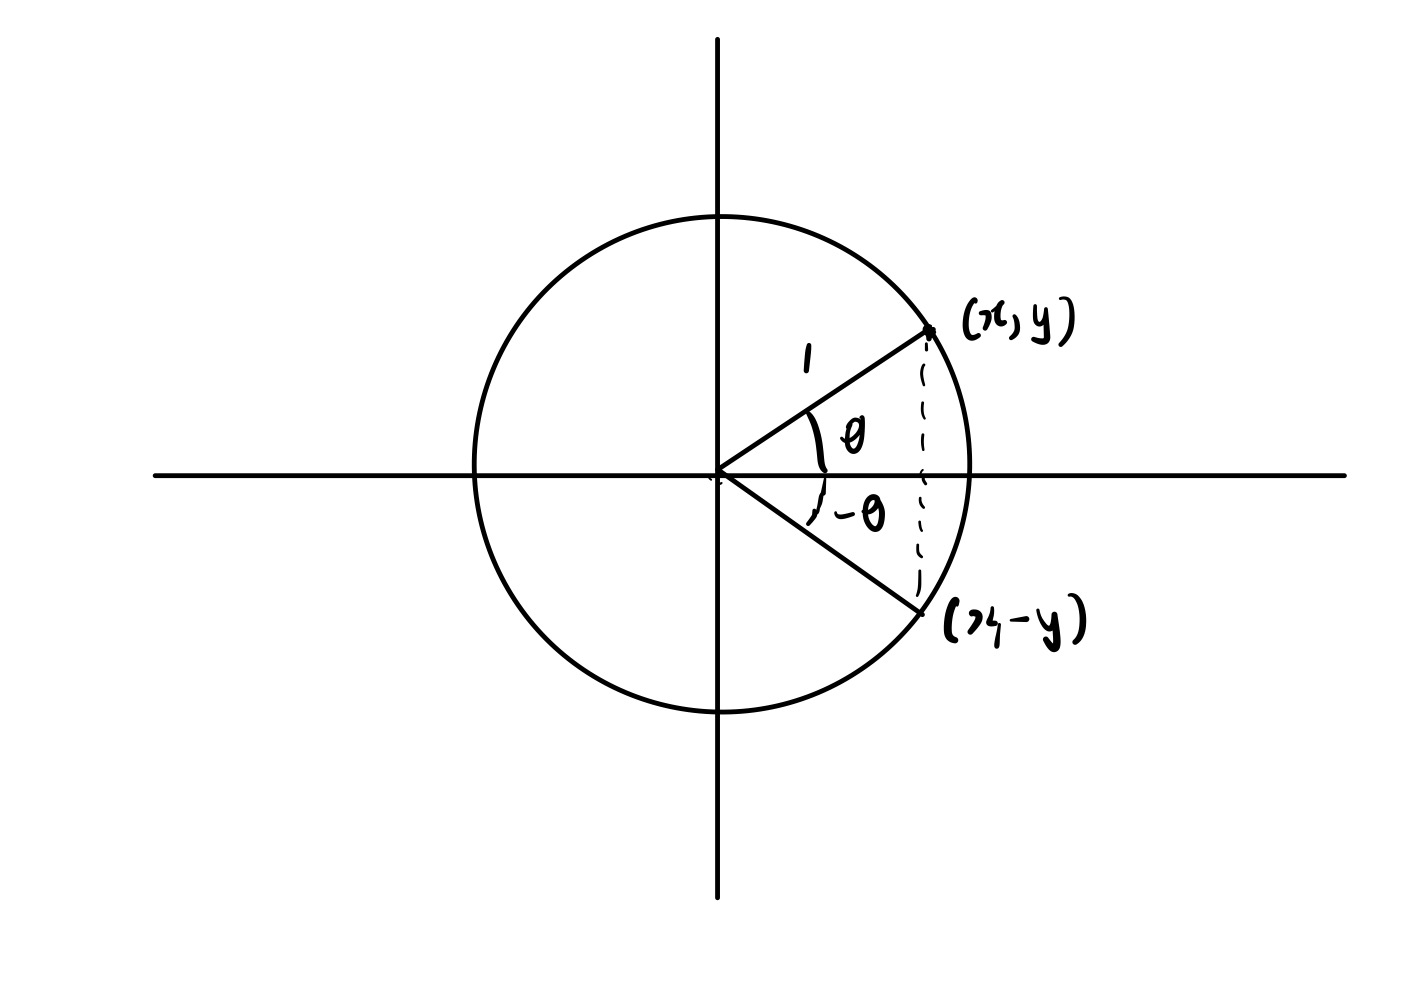
\includegraphics[width=\textwidth]{unit_circle.jpg}

\textit{(b)}
\begin{proof}
    Considering the Cartesian plane, $\theta$ is the angle formed by the x-axis and
    a line from the origin to a point $(x,y)$, measured counterclockwise from the x-axis.
    Thus, $-\theta$ is the same angle, measured from the same point reflected on the x-axis.

    Reflecting $(x,y)$ on the x-axis corresponds to the following transformation:
    \[
        (x,y) \rightarrow (x,-y)
    \]
    Since $\cos(\theta) = x$, $\cos(-\theta)$ is the x-coordinate of the point reflected
    on the x-axis, which is $x$.
\end{proof}

\textit{(c)}
\begin{proof}
    Considering (b), a reflection of $\theta$ on the x-axis corresponds to the transformation
    of $(x,y) \rightarrow (x,-y)$.
    Since $sin(\theta) = y$, $sin(-\theta)$ is the y-coordinate of the point reflected
    on the x-axis, which is $-y$.
\end{proof}
\end{document}